%
% Niniejszy plik stanowi przykład formatowania pracy magisterskiej na
% Wydziale MIM UW.  Szkielet użytych poleceń można wykorzystywać do
% woli, np. formatujac wlasna prace.

% Zawartosc merytoryczna stanowi oryginalnosiagniecie
% naukowosciowe Marcina Wolinskiego.  Wszelkie prawa zastrzeżone.
%
% Copyright (c) 2001 by Marcin Woliński <M.Wolinski@gust.org.pl>
% Poprawki spowodowane zmianami przepisów - Marcin Szczuka, 1.10.2004
% Poprawki spowodowane zmianami przepisow i ujednolicenie 
% - Seweryn Karłowicz, 05.05.2006
% Dodanie wielu autorów i tłumaczenia na angielski - Kuba Pochrybniak, 29.11.2016

% dodaj opcję [licencjacka] dla pracy licencjackiej
% dodaj opcję [en] dla wersji angielskiej (mogą być obie: [licencjacka,en])
\documentclass[licencjacka]{pracamgr}

\usepackage{graphicx,xcolor,listings}

% Dane magistranta:
%\autor{Imię Nazwisko}{123456}


% Dane magistrantów:
\autor{Daniel Gutowski}{372207}
\autori{Jakub Kuklis}{371125}
\autorii{Adrian Naruszko}{371233}
\autoriii{Filip Plata}{371335}

\title{Modernizacja architektury autorskiego CMS firmy e-point}


\kierunek{informatyka}

\opiekun{mgr. Krzysztofa Wojciecha Ciebiery\\
  Instytut Informatyki\\
  }

\date{Kwiecień 2018}

\dziedzina{ 
11.3 Informatyka
}

%Klasyfikacja tematyczna wedlug AMS (matematyka) lub ACM (informatyka)
\klasyfikacja{D. Software\\
  D.1.5. Object-oriented Programming\\
  D.2.5. Testing and Debugging\\
  D.2.7: Distribution, Maintenance, and Enhancement\\
  D.2.10: Design\\
  D.2.11: Software Architectures\\
  }

% Słowa kluczowe:
\keywords{CMS, Java, ORM, rendering, modernizacja, Jooq, Gatling, Caffeine, cache, Jooq, ACN}


\newtheorem{defi}{Definicja}[section]


\begin{document}

\maketitle

\begin{abstract}
  W~pracy przedstawiamy opis współpracy w firmą e-point.
  Produktem nad którym pracowaliśmy, jest autorski
  system CMS. W momencie rozpoczęcia współpracy miał on strukturę monolitu.
  Naszym zadaniem było napisanie mikroserwisów umożliwiających
  dalszą modernizację i modularyzację tego produktu. 
  Ostatecznie zajmowaliśmy się komponentami odpowiadającymi za dostęp do bazy danych oraz rendering.
  Celem jest wkomponowanie starego systemu w nowy jako jego część.
\end{abstract}

\tableofcontents

\chapter*{Wprowadzenie}
\addcontentsline{toc}{chapter}{Wprowadzenie}

Jednym z powszechnych problemów wśród dużych firm prowadzących wieloletnią działalność  jest przestarzałość części wykorzystywanych rozwiązań. Metodyki w branży stale ewoluują, wciąż pojawiają się nowe, coraz lepsze sposoby radzenia sobie z rozpatrywanymi zagadnieniami, w związku z czym bez odpowiednio regularnie przeprowadzanych modernizacji systemów trudno nadążać za konkurencją. Szczególnie dotyka to przedsiębiorstw stawiających na autorskie rozwiązania - rynek wytwarza nowe komponenty i narzędzia szybciej, niż jest to w stanie zrobić pojedyncza firma, a modernizacja wiąże się zwykle z dużymi kosztami wynikającymi przede wszystkim ze stopnia złożoności i liczby wzajemnych zależności w istniejących strukturach. 

\vspace{1mm}

Branża usług sieciowych nie stanowi tutaj wyjątku. Stale rosnąca liczba frameworków i częste zmiany w podejściu do tworzenia serwisów internetowych wymuszają konieczność dbania o aktualność używanych rozwiązań. E-point to jedna z firm, która stanęła przed problemem modernizacji swojego systemu - autorskiego CMS o nazwie ACN. Zadanie to powierzyła w części naszemu zespołowi.

\vspace{1mm}

W szczególności, zajmowaliśmy się implementacją dwóch mikroserwisów:
\begin{enumerate}
\item DataAPI - RESTowa aplikacja integrująca bazę danych aktualnego CMSa z nowym mechanizmem renderingu.
\item Element odpowiedzialny za rendering stron internetowych na podstawie szablonów oraz związana z nim architektura.
\end{enumerate}

\chapter{Zarys sytuacji i historia problemu}

W tym rozdziale omówiona zostanie działalność firmy e-point, struktura ACN oraz wynikające z niej problemy.

\begin{center}

\includegraphics[scale=0.52]{images/logo.JPG}
\end{center}

\section{Firma e-point}

E-point to polskie przedsiębiorstwo zajmujące się tworzeniem oprogramowania, dostarczające systemy internetowe dla międzynarodowych korporacji oraz usługi w modelu SaaS (software as a service). Założone w 1996 roku, działa nieprzerwanie od ponad 20 lat, otrzymując za swoją działalność liczne nagrody i wyróżnienia od przedstawicieli branży technologicznej. Jej klientami są największe firmy polskie i zagraniczne, takie jak ING Bank Śląski, Bank BGŻ BNP Paribas czy Amway.

Działalność firmy koncentruje się na następujących sektorach:
\begin{itemize}
\item systemy e-commerce – aplikacje mające na celu sprzedaż produktów i usług oraz zapewnienie obsługi klientów i partnerów przez internet – sklepy internetowe, bankowość elektroniczna, eCRM, systemy obsługi zamówień
\item portale korporacyjne – systemy mające na celu udostępnianie informacji na zewnątrz i wewnątrz organizacji – serwisy WWW, portale wewnętrzne, extranety
\item aplikacje mobilne aplikacje i serwisy na smartfony i tablety
\item systemy e-wniosków – rozwiązania zorganizowane wokół zagadnienia zbierania i przetwarzania wniosków (formularzy elektronicznych)
\item systemy mające na celu obsługę wybranych procesów biznesowych w organizacji – rejestry, wsparcie sprzedaży, operacyjne CRM, e-learning
\end{itemize}

W czasie tylu lat istnienia e-point wypuścił na rynek wiele swoich własnych produktów, m.in. kreator stron mobilnych ActiveMobi, modeler baz danych Vertabelo czy OneWebSQL, pierwsze polskie narzędzie do mapowania obiektowo-relacyjnego – sposobu odwzorowania obiektowej architektury systemu informatycznego na bazę danych o relacyjnym charakterze. Nasze zadania związane były z wewnętrznym CMS, używanym do zarządzania danymi i renderowania odpowiednich treści w serwisach internetowych klientów firmy.

\section{ACN}

ACN - wewnętrzny CMS (Content Management System) - to jeden z największych produktów firmy. Odpowiada za cały proces utrzymywania, przygotowania i serwowania danych serwisom internetowym. W momencie otrzymania zapytania load balancer decyduje o przekierowaniu go do odpowiednio odciążonego serwera. Request trafia do ACN, który po pomyślnej weryfikacji uprawnień dostępu wyciąga dostępne komponenty z cache’u, a o informacje potrzebne do przetworzenia pozostałych odpytuje bazę danych. W dalszej kolejności renderowane są niecache’owalne elementy strony oraz te nieobecne w danym momencie w cache’u. Po wygenerowaniu wszystkich potrzebnych komponentów strona jest serwowana użytkownikowi.

\section{Problemy obecnej architektury}
Dotychczas ACN stanowił monolit. Jest to produkt tworzony od wielu lat, stale rozwijany i rosnący. W samej bazie danych część zmian podyktowana była indywidualnymi wymaganiami klientów, przez co stała się ona mało przejrzysta i trudna w utrzymaniu. Duża wielkość systemu sprawia, że jego modyfikacja jest uciążliwa – zachowanie spójności wszystkich usług przy nawet pozornie małych zmianach wymaga wielu godzin pracy nad kodem. Utrudniona jest także lokalizacja błędów w systemie, brak modułowości oznacza konieczność przeszukiwania znacznie większej ilości kodu w celu wykrycia usterki. Kolejną przeszkodą jest brak automatycznych testów oraz systemu ciągłej integracji, a co za tym idzie - brak sprecyzowanego wyznacznika poprawnego działania systemu. Spięcie wielu różnych technologii w jedną całość znacznie utrudnia pracę wszystkim narzędziom do statycznej analizy kodu.

\vspace{1mm}

Problem stanowi również framework, na którym oparty jest ACN. Kilkanaście lat temu, gdy system dopiero powstawał, nie były dostępne jeszcze tak dopracowane rozwiązania, jak te oferowane obecnie na przykład przez framework Spring. W firmie zdecydowano się na stworzenie własnej platformy, tak rozpoczęła się praca nad OneWeb'em, do tej pory stanowiącym podstawę ACN'a. Z biegiem czasu zapotrzebowanie na ogólnodostępne narzędzia stało się jednak na tyle duże, że autorskie rozwiązanie nie było w stanie konkurować z dynamicznie rozwijającymi się alternatywami. Ostatecznie firma podjęła decyzję o migracji na Spring, której początkowy etap mieliśmy zrealizować.

\vspace{1mm}

W związku z przejściem do bardziej nowoczesnego podejścia pojawił się pomysł przynajmniej częściowego wydzielenia funkcjonalności ACN do osobnych mikroserwisów. Implementacja dwóch z nich, elementu łączącego aplikację z bazą danych oraz serwisu renderującego komponenty strony, została przydzielona naszemu zespołowi.

\chapter{Koncepcja modernizacji}

W tym rozdziale przedstawiona zostanie wstępna faza prac oraz wizja tego, jak ma wyglądać system ACN po modernizacji.
	
\section{Początek prac – inny projekt}

Założenia naszego projektu nie były od początku jasne. Pierwotnie mieliśmy zająć się innym zadaniem – zaimplementowaniem personalizacji treści serwisów internetowych na podstawie aktywności ich użytkowników. Miało to pozwolić przede wszystkim na bardziej trafne wyświetlanie ofert i reklam. Po wstępnej konfiguracji dostępów i tunelowania zdążyliśmy stworzyć podstawową architekturę aplikacji i skonfigurować narzędzie deweloperskie na AWS, kiedy okazało się, że rozwój produktu zostaje wstrzymany ze względu na problemy z jego sprzedażą. Wtedy też przedstawiciele firmy podjęli decyzję, że nasz projekt będzie w całości poświęcony modernizacji aktualnie funkcjonującego systemu. 

\section{Ostateczny projekt}
	
Rozwiązanie zaproponowane i wdrażane przez firmę ma opierać się na stylu programowania REST, tj. wykorzystującym predefiniowane bezstanowe operacje, co pozwala osiągać dużą wydajność, modułowość i niezawodność aplikacji. Docelowo pojawić mają się następujące mikroserwisy:
\begin{itemize}
\item frontend - przyjmowanie zapytań i serwowanie stron WWW;
\item rendering - tworzenie stron na podstawie szablonów, wykorzystuje usługi udostępniane przy pomocy serwisu Registry;
\item AC Data API - abstrakcja bazy danych, udostępnia tylko niezbędne renderingowi dane;
\item Registry - rejestr wewnętrznych i zewnętrznych usług takich jak podmiana tagów, personalizacja treści;
\item ACN - dotychczasowa aplikacja implementująca niektóre usługi, w końcowym etapie ma zniknąć.
\end{itemize}

Nasza grupa zajmowała się elementami Data API oraz serwisem renderującym. W przypadku tego drugiego, część pracy stanowiło wprowadzenie zmian w samym ACN, związanych z dostosowywaniem narzędzia do nowej koncepcji schematu renderowania. Dodatkowym wyzwaniem było założenie, że na każdym etapie prac nasze rozwiązanie ma współistnieć z dotychczasowym, przejmując po kolei jego obowiązki.

\vspace{30mm}

\begin{figure}[h]
	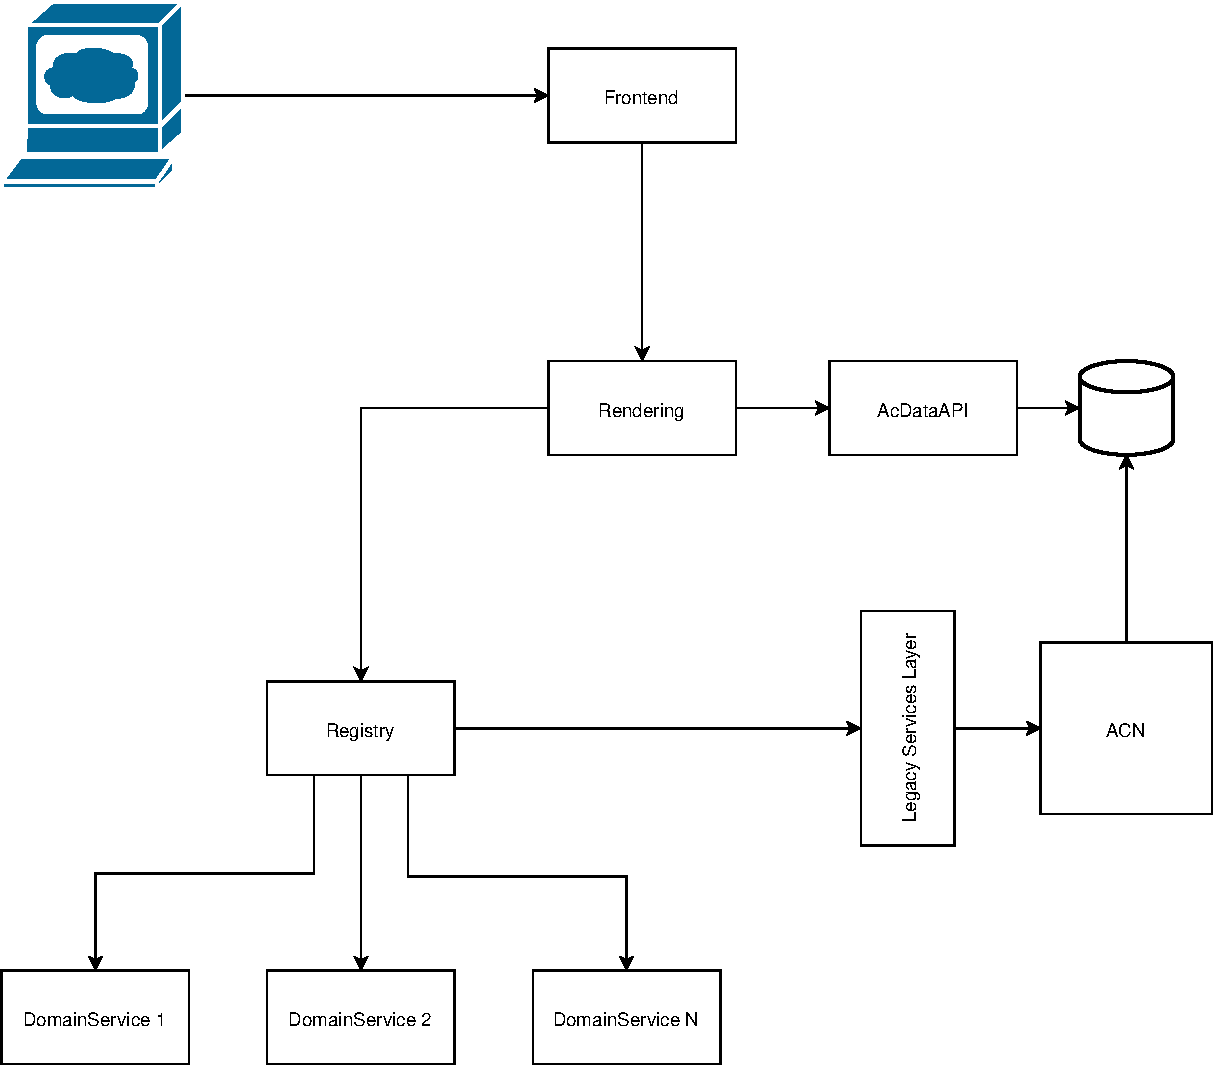
\includegraphics[scale=0.82]{images/architecture.pdf}
	\caption{Schemat wydzielonych aplikacji}
\end{figure}

\chapter{AC Data API}

W tym rozdziale przeanalizowana zostanie struktura ACN i bazy danych oraz przedstawione zostaną założenia naszego projektu.

\section{Mikroserwis}

Obsługa serwisów internetowych wymaga niezawodnego i bezpiecznego sposobu łączenia z bazą danych, dobrym pomysłem wydaje się więc wydzielenie odpowiedniego mikroserwisu odpowiedzialnego za to zadanie. E-point korzysta z tradycyjnych relacyjnych baz danych, co pociąga za sobą stosowanie ORM przy wyciąganiu danych do dalszego przetwarzania. Dzięki wydzieleniu takiej usługi możliwe jest także uniknięcie zauważonych w ACN błędów w strukturze bazy danych - mikroserwis pośredniczący pozwala na wyabstrahowanie prawdziwego rozkładu tabel i pól w bazie, dzięki czemu w przyszłości będzie można zmienić również schemat bazy danych.

\vspace{1mm}

Aplikacja Data API ma udostępniać dane z bazy danych ACN dla komponentów w nowej architekturze. Będzie to jeden z najczęściej odpytywanych serwisów, w związku z czym jego wydajność oraz dostępność jest krytyczna dla sprawnego i poprawnego działania całej usługi.

\section{Założenia}

Aplikacja docelowo ma specyfikować oraz implementować kontrakt obsługi REST’owych endpointów, których nazwy składają się z wersji API oraz tytułu zapytania (np. /v1/language-version). Odpowiedzią na dane żądanie jest JSON zawierający odpowiednie dane z bazy.

\vspace{1mm}

Dane z bazy danych mają być zapisywane w odpowiednio inwalidowanym cache’u. Powodem inwalidacji może być upływ wyznaczonego czasu od zapisu czy powiadomienie o zmianie z innego serwisu połączonego z bazą danych (na ten moment funkcję tę pełni ACN).

\vspace{1mm}
	
API ma być dokładnie pokryte testami, zarówno poprawnościowymi, jak i wydajnościowymi. Nie jest wymagana żadna forma uwierzytelniania dostępu.

\vspace{1mm}

Kluczowa jest struktura kodu, która umożliwia płynne  zmienianie wersji API, z zachowaniem wstecznej kompatybilności poprzednich wersji API. Główną trudnością są tutaj zmiany w schemacie bazy danych.

\section{Struktura bazy}

Baza danych składa się z wielu schematów. Głównym schematem jest schemat ‘master’. Przechowuje on informacje o klientach – organizacjach – korzystających z systemu firmy e-point. Dla każdego klienta tworzony jest schemat identyfikowany jego kodem ('common-*'), zawierający np. informacje o użytkownikach zarejestrowanych w serwisach tegoż klienta. Dla każdego portalu zarządzanego przez organizację tworzony jest osobny schemat ('site-*'), w którym przechowywane są wszystkie dane dotyczące instancji portalu.

\section{Użyte technologie}

Aplikacja została napisana w Javie w wersji 8 przy użyciu platformy Spring. Ostatecznie przy jej tworzeniu korzystaliśmy m.in. z:
\begin{itemize}
\item systemu automatycznego budowania Gradle;
\item pakietu Jooq (Java Object Oriented Querying), lekkiej biblioteki ORM;
\item biblioteki Caffeine, służącej do cache’owania;
\item Elastic Stacka, na którym oparliśmy system służący do monitorowania działania aplikacji;
\item platformy Docker z postgresem do testowego uruchomienia aplikacji;
\item frameworku Gatling, stosowanego przy tworzeniu i wykonywaniu scenariuszy testów wydajnościowych;
\item funkcjonalności związanych z IntelliJ IDEA.
\end{itemize}

\chapter{Praca nad AC Data API}

W tym rozdziale opisana zostania praca wykonana przy tworzeniu AC Data API.

\section{Iteracja nr 1}

W pierwszej iteracji do generowania klas Javy na podstawie schematów z bazy danych użyliśmy pakietu Jooq. Zaprezentowany przez nas przykład rozwiązania oparty bardzo bezpośrednio na Jooqu został odrzucony przez naszych przełożonych ze względu na ujawnione braki w architekturze rozwiązania. Problematyczne okazało się m.in. zapewnienie ścisłego, sztywnego kontraktu przez API przy zmianach schematów w bazie danych.

\vspace{1mm}

Ujawnione wady wcześniejszej koncepcji spowodowały przestój w pracach związany z dyskusją nad możliwościami rozwiązania wykrytych problemów. Po dogłębnej analizie dostępnych narzędzi i prezentowanych przez nas demonstracyjnych kawałków kodu nasz przełożony zdecydował się na pozostaniu przy pakiecie Jooq, z tą różnicą, że warstwa aplikacji zależna od Jooq miała zostać wydzielona od pozostałej części kodu, niezależnej od sposobu dostępu do bazy danych.

\vspace{1mm}

W tej wersji do monitorowania aktywnych instancji aplikacji użyliśmy gotowego, dedykowanego narzędzia spring-boot-admin. Niestety, konfiguracja narzędzia okazała się tyleż prosta, co ograniczona. Nie mogąc spełnić wymogów firmy przy jego pomocy, zdecydowaliśmy się na inny produkt do monitorowania aplikacji.
	
\section{Iteracja nr 2}

Ta iteracja poświęcona była przede wszystkim na poprawne zaimplementowanie ORM oraz stworzenie potrzebnych endpointów. Przyjęliśmy architekturę podzieloną na kilka warstw odpowiedzialnych za wydzielone zadania. 

\vspace{1mm}

Najniższa z nich zapewnia bezpośredni dostęp do bazy danych poprzez Jooq. Druga warstwa zajmuje się dzieleniem danych klientów na schematy w bazie, zarządzaniem aktualnymi schematami - jej implementacja opiera się na wykorzystaniu aspektów. Następny poziom ukrywa działanie Jooq’a poprzez utworzenie obiektów domenowych. Ostatecznie wersjonowanie API poprzez javowe pakietowanie umożliwia zapewnienie kontraktu kompatybilnego wstecz nawet pomimo zmian schematu bazy danych.

\vspace{1mm}

Odpowiednie endpointy realizują zapytania potrzebne wyższym poziomom obsługi żądań do stron. Listę niezbędnych zapytań przygotowali nasi przełożeni. Wśród zaimplementowanych endpointów znajdują się m.in. zapytania pobierające wersje językowe, informacje o kliencie o zadanym identyfikatorze czy własności strony o zadanym id. Wszystkie te metody obłożone są testami poprawnościowymi napisanymi przy pomocy JUnit.

\section{Iteracja nr 3}

Mając zaimplementowaną strukturę aplikacji, przystąpiliśmy do zadań związanych z jej wydajnością. Pierwszym krokiem była konfiguracja cache’u. Na podstawie analizy dostępnych w internecie źródeł i benchmarków zdecydowaliśmy się na Caffeine, bardzo wydajną bibliotekę do cache’owania oparta na Javie 8.

\vspace{1mm}

Spring dobrze współdziała z różnymi frameworkami i Caffeine nie jest tu wyjątkiem. Wybór elementów do cache’owania odbywa się poprzez dodanie odpowiednich adnotacji przy cache’owanych funkcjach – model zmian w kodzie przy pomocy adnotacji to zresztą powszechny w Springu mechanizm.

\vspace{1mm}

Gotowy cache poddaliśmy testom wydajnościowym generowanym przy pomocy scenariuszy korzystających z Gatlinga.

\vspace{1mm}

Działanie całej aplikacji możemy monitorować, korzystając z Elastic Stacka. Wymaga on wprawdzie ręcznego wprowadzania reguł dla oczekiwanych statystyk i nie radzi sobie najlepiej z agregowanymi danymi, zapewnia za to pełną konfigurowalność. Będąca częścią Elastic Stacku Kibana pozwala nam na graficzną reprezentację zebranych statystyk, poniżej przykładowe wynikowe wykresy.

\vspace{15mm}

\begin{figure}[h]
	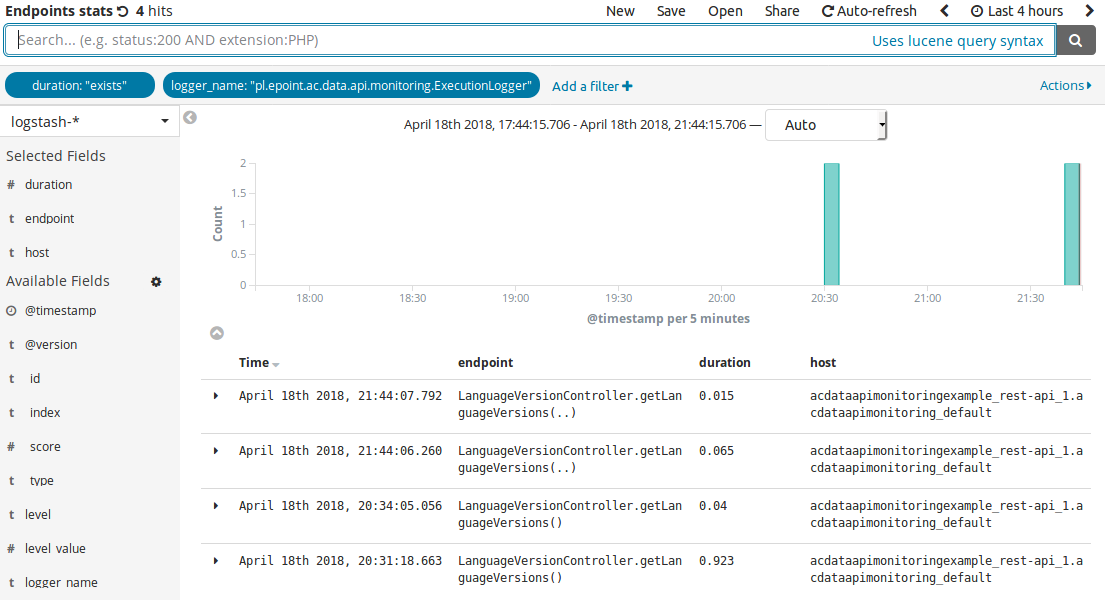
\includegraphics[scale=0.38]{images/kibana2.png}
	\caption{Interfejs Kibany}
\end{figure}
\begin{figure}[h]
	\centering
	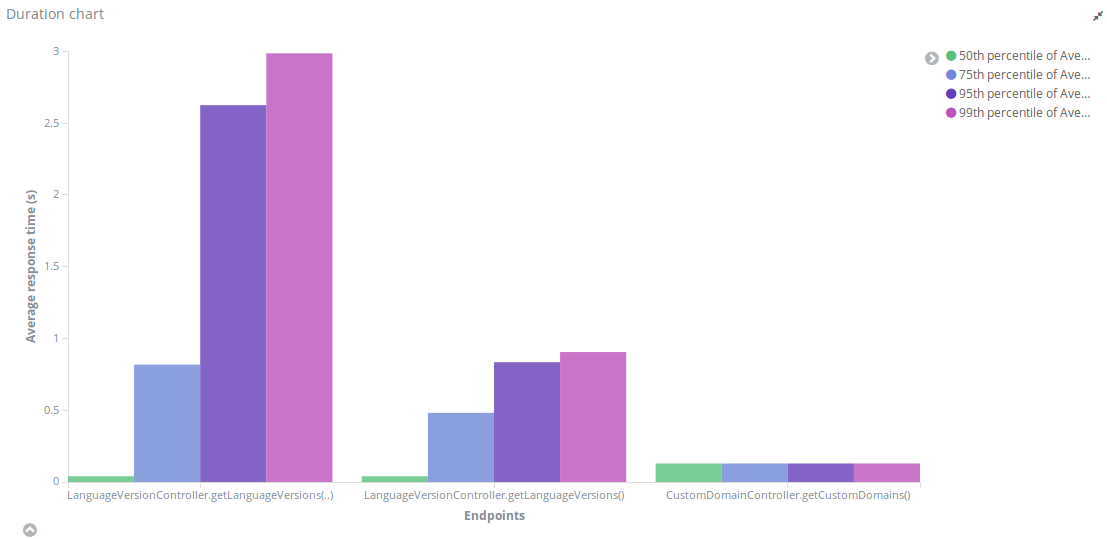
\includegraphics[scale=0.38]{images/kibana3.png}
	\caption{Wykresy średniego czasu odpowiedzi na zapytania}
\end{figure}
\begin{figure}[h]
	\centering
	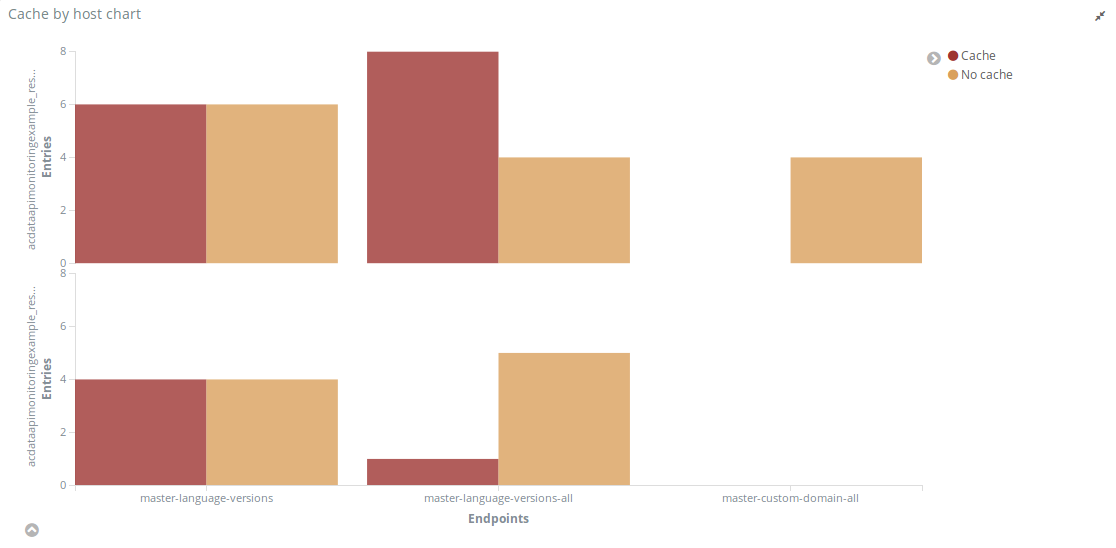
\includegraphics[scale=0.38]{images/kibana4.png}
	\caption{Wykresy dotyczące wykorzystania cache'u}
\end{figure}

\chapter{Rendering}

W tym rozdziale opisana zostanie wizja nowego mechanizmu renderingu oraz wykonana przez nas praca przy architekturze potrzebnej do jego wprowadzenia.

\section{Rendering przed modernizacją}

W dotychczasowym modelu renderowania można było wydzielić dwa etapy wykonywane odpowiednio przed i po sięgnięciu do cache'u. ACN wykorzystuje poza tym także komponenty z ustawionym w bazie danych parametrem ‘noncacheable attributes’. Elementy te miały swoje wersje w cache’u zależne od parametru żądania (zazwyczaj) czy też ciasteczka pochodzącego z sesji. 
Całość renderowania wykonywana była przez ACN, co ograniczało wydajność systemu. Taka struktura powodowała, że przeglądarka klienta i jej cache pozostawały niewykorzystane.

\vspace{1mm}

W rozwiązaniu wdrażanym przez firmę opisany wyżej postprocessing ma docelowo zniknąć. Naszym zadaniem było takie przystosowanie ACN, które pozwoliłoby na przeniesienie części renderingu do przeglądarki użytkownika. Powiązanym celem było rozdzielenie frontendu i backendu tak, by łączyło je tylko API. Pozwala to na użycie jednego z nowoczesnych framerowków do tworzenia interfesju ACN. 

\vspace{1mm}	
	
Dopiero po wykonaniu powyższego zadania możliwe było przystąpienie do pisania nowego komponentu renderującego.

\section{Iteracja nr 1}
	
Pierwszym etapem naszej pracy była konfiguracja środowiska potrzebnego do testowania wprowadzanych przez nas zmian. Początkowo do sprawdzania działania nowej implementacji zamierzaliśmy używać kontenera LXD, niestety nie udało się w nim uruchomić aplikacji - wymagania techniczne ACN nie są nigdzie precyzyjnie sformułowane i nie jesteśmy w stanie stwierdzić, czego konkretnie brakowało aplikacji. Ostatecznie postanowiliśmy przechowywać całe środowisko na maszynie wirtualnej. Do obsługi serwera używany jest Apache oraz JBoss. Dla usprawnienia pracy korzystamy także z JRebela, narzędzia pozwalającego na aktualizowanie kodu i obserwowanie zmian bez restartowania serwera.

\vspace{1mm}

W tym czasie nasi przełożeni przygotowywali zmiany w komponentach powiązanych z ACN, takich jak OneWeb, by umożliwić nam pracę nad serwisem renderującym. Jedną z istotnych zmian było umożliwienie cache’owania formularzy. Uczenie się obsługi OneWeba była kolejną rzeczą, która zajmowała nas w tej części.
	
\section{Iteracja nr 2}

W tej iteracji naszym zadaniem było wyczyszczenie ACN z elementów uznanych przez naszych przełożonych za zbędne – bardzo rzadko używanych i stosunkowo łatwo podmienialnych lub niecache’owalnych. Wyspecyfikowanych zostało również kilkanaście komponentów wymagających poprawek. Mieliśmy wprowadzić do nich takie modyfikacje, aby całe komponenty były cache’owalne, a treści, które do tej pory w tym przeszkadzały, pobierane były poprzez JavaScript już po wyświetleniu głównej części strony.

\chapter{Podział pracy}

W tym rozdziale każdy z nas opisuje, czym zajmował się w projekcie.

\section{Daniel Gutowski}

W trakcie pracy nad AC Data API zajmowałem się wyborem i konfiguracją biblioteki ORM. Rozważałem przede wszystkim biblioteki JOOQ oraz Hibernate. Obie wspierają generowanie klas JAVowych na podstawie schematu bazy danych oraz umożliwiają łatwe pisanie zapytań SQL. O wyborze JOOQ'a zdecydowała łatwość w przełączaniu się pomiędzy schematami, możliwość generowania kodu na podstawie danych udostępnianych przez Vertabelo oraz jego popularność.
Poza tym napisałem logikę trzech endpointów wystawianych przez aplikację oraz zintegrowałem narzędzie generujące opis API RESTowego (format OpenAPI), na podstawie którego można wygenerować kod do łatwego korzystania z aplikacji.

\vspace{1mm}

W ramach modularyzacji ACN pracowałem nad mechanizmem renderowania linków kanonicznych. Jest to informacja zawarta w kodzie strony, która mówi robotowi wyszukiwarki internetowej o właściwym adresie internetowym tej strony. Dotychczas był to element postprocessingu, ponieważ w linkach zawarta jest informacja o parametrach, które nie są częścią klucza cache. Wymagało to przeniesienia całej logiki na stronę przeglądarki i umieszczenia wewnątrz HTMLa danych opisujących renderowanie, takich jak lista parametrów strony stanowiących część linku czy nazwa domeny.

\vspace{3mm}

\section{Jakub Kuklis}

W ramach pracy nad AC Data API zajmowałem się analizą działania cache'u i wyborem oraz konfiguracją odpowiedniego frameworku do tego zagadnienia. Najbardziej obiecującymi platformami wydały mi się Redis, z którym nasz zespół miał już styczność, EhCache, sprawdzone i efektywne rozwiązanie, oraz Caffeine, jedna z nowszych platform. Ostatecznie na podstawie dostępnych benchmarków, swoich testów i porównania wsparcia w Springu wybrałem Caffeine do naszego projektu. Poza tym pracowałem nad wystawianymi przez API endpointami oraz asystowałem przy testowaniu ElasticStacka.

\vspace{1mm}

Podczas modernizacji architektury renderingu zająłem się kodem komponentów występujących pod wspólną etykietą "Quotes". Komponenty te były wykorzystywane na tyle rzadko, że nasi przełożeni zdecydowali o ich usunięciu, należało więc wyczyścić kod z ich wystąpień.

\vspace{1mm}

Dodatkowo jestem odpowiedzialny za część obowiązków niezwiązanych z pracą dla firmy, takich jak ostateczny kształt pracy licencjackiej czy plakat projektu.

\section{Adrian Naruszko}

W trakcie pracy nad AC Data API zajmowałem się bazową konfiguracją projektu, stworzeniem zalążka projektu i dodaniem niezbędnych do pracy narzędzi. 
Zintegrowałem z projektem framework do tworzenia i wykonywania scenariuszy do testów wydajnościowych - Gatling. 
Framework ten pozwala na symulowanie zachowań użytkowników na działającej aplikacji.
Kolejnym etapem mojej pracy było zintegrowanie ElasticStacka do monitorowania zachowania instancji Data API. W ostatecznym rozwiązaniu użyłem następujących narzędzi:
\begin{itemize}
\item ElasticSearch - backend systemu analizujący wszystkie dane;
\item MetricBeat - odpytuje w stałych interwałach czasowych różne endpointy aplikacji, np. /health czy /metrics, które dostarczają odpowiednie statystyki;
\item Logstash - pośredniczy w przesyłaniu logów aplikacji do ElasticSearcha, filtruje je lub przystosowuje ich schemat;
\item Kibana - frontend prezentujący zapytania ElasticSearcha w formie wykresów, tabel.
\end{itemize}

\vspace{1mm}

Podczas modyfikowania kodu ACN przystosowywałem do nowego rozwiązania kod kontrolerów, które dotychczas były cache'owane tylko częściowo.

\vspace{10mm}

\section{Filip Plata}

Początkowo mieliśmy robić inny projekt - w związku z tym wykonałem wiele koniecznych prac, takich jak zestawienie systemów deweloperskich na AWS oraz nieduży PoC.

Większą część swojego wysiłku włożyłem w pracę nad Data API. W początkowej fazie dostarczyłem kilka różnych wersji kodu, które pomagały sprecyzować oczekiwania firmy co do tego mikroserwisu. Wtedy też okazało się, że konieczne jest wspieranie starej wersji API po zmianie bazy danych.

Proces tworzenia kodu endpointu był powtarzany, aż uzyskany komponent spełniał wszystkie wymagania naszych przełożonych, czasem zmieniane na podstawie ujawnionych wad wcześniejszych koncepcji. Od strony technicznej szczególnie ciekawy wydaje się kod służący do zarządzania aktualnym schematem używanym przez Jooq. Został on zrealizowany jako aspekt we frameworku Spring Boot, gdyż bardzo dobrze wpasował się w ten paradygmat. Za pomocą odpowiednich adnotacji wstrzykujemy logikę odpowiedzialną za ustawienie konkretnego schematu, z którego będą pobierane dane.

\vspace{1mm}

W czasie pracy nad ACN skupiłem się głównie na próbie postawienia go w powtarzalny sposób w kontenerze LXD. Próba ta zakończyła się niepowodzeniem, ale ostatecznie udało się stworzyć odpowiednią maszynę wirtualną i wypracować dość efektywny sposób pracy z kodem systemu.

\newpage
Poniżej wycinek kodu z projektu DataAPI zarządzający schematami:

\begin{lstlisting}
@Aspect
@Component
@RequiredArgsConstructor
class SchemaAspect {

    private final SchemaUtilsService schemaUtilsService;

    @Around("@annotation(pl.epoint.ac.
    data.api.infrastructure.ClientSchemaQuery) && args(clientId,..)")
    public Object setClientSchema(ProceedingJoinPoint joinPoint, 
          String clientId) throws Throwable {
        schemaUtilsService.beforeClientSchemaQuery(clientId);
        Object proceed = joinPoint.proceed();
        schemaUtilsService.afterClientSchemaQuery();

        return proceed;
    }

    @Around("@annotation(pl.epoint.ac.
    data.api.infrastructure.SiteSchemaQuery) && args(siteId,..)")
    public Object setSiteSchema(ProceedingJoinPoint joinPoint, 
          Integer siteId) throws Throwable {
        schemaUtilsService.beforeSiteSchemaQuery(siteId);
        Object proceed = joinPoint.proceed();
        schemaUtilsService.afterSiteSchemaQuery();

        return proceed;
    }
}

// SchemaUtilsService - example method

private void setSchemaMapping(String inputMapping, 
      String outputMapping) {
    Collection<MappedSchema> mapping = Collections
            .singleton(new MappedSchema()
                    .withInput(inputMapping)
                    .withOutput(outputMapping));

    dslContext.settings().setRenderMapping(new RenderMapping()
        .withSchemata(mapping));
}
\end{lstlisting}


\begin{thebibliography}{99}
\addcontentsline{toc}{chapter}{Bibliografia}

\bibitem[Wiki18]{wikipedia} Wielu autorów, \textit{E-point}, pl.wikipedia.org/wiki/E-point, 2018.



\end{thebibliography}


\end{document}
